\documentclass[11pt]{article}

\usepackage[margin=1in]{geometry}
\usepackage{amsmath}
\usepackage{booktabs}
\usepackage{float}
\usepackage{graphicx}
\usepackage{hyperref}
\usepackage{microtype}
\usepackage{xcolor}

\hypersetup{
  colorlinks=true,
  linkcolor=blue!45!black,
  urlcolor=blue!55!black,
  citecolor=blue!45!black,
  hypertexnames=false
}

\graphicspath{{../../work-packages/20260809_peakflow_topanga_census_execution/artifacts/}}

\newcommand{\Ksat}{\ensuremath{K_{\mathrm{sat}}}}
\newcommand{\PeakRO}{\texttt{PeakRO}}
\newcommand{\surdra}{\texttt{surdra}}

\title{Small-Mutation Screening of WEPP Hillslope Peak Flow\\
\large Methodology and Interim Topanga Results}
\author{Roger Lew\thanks{University of Idaho; report prepared with agentic coauthor support from OpenAI Codex.}}
\date{Version 0.1 --- August 9, 2026}

\begin{document}
\maketitle

\begin{abstract}
This report describes a controlled, full-history screening experiment designed
to detect discontinuous responses in the Water Erosion Prediction Project
(WEPP) hillslope peak-flow estimate. The experiment perturbed first-horizon
saturated hydraulic conductivity by only $-1\%$ or $+1\%$, or changed paired
interrill and rill cover by only $-0.01$ or $+0.01$. Each run changed one
hillslope and one parameter family while holding the scenario, climate,
topography, antecedent simulation history, and all other inputs fixed.

The Topanga census completed 1,088 eligible mutation trials across burned and
unburned scenario strata. The combined event record contains 225,654 rows from
the baseline and mutant runs, of which 225,036 could be matched directly.
Preregistered screening rules flagged
11,506 event rows (5.10\%) distributed across 1,027 trials. The result is
strongly structured by parameter family: all 560 \Ksat{} trials contained at
least one candidate event, and the \Ksat{} event-row candidate rate was 8.62\%,
compared with 1.33\% for cover.

Event runoff depth is highly stable under the small probes: only 451 of 218,985
paired-positive runoff rows (0.21\%) lie outside a mutant-to-baseline ratio of
0.5--2, and 98.3\% of \Ksat{} runoff responses have the expected inverse sign.
Event sediment delivery is also mostly controlled: only 271 of 139,255
paired-positive rows (0.195\%) lie outside 0.5--2. The retained sediment output
is quantized to 0.1 kg/m, however, and substantial relative scatter remains at
small magnitudes and within the central band.
Peak flow is less stable. Of 199,086 plotted paired-positive peak rows, 989
(0.50\%) lie
outside a mutant-to-baseline ratio of 0.5--2, and 604 (0.30\%) lie outside
0.2--5---an empirical rate of approximately one event row in 330. More than
91\% of both tails are \Ksat{} mutations. Most extreme
responses have the ordinary hydrologic sign---lower \Ksat{} raises peak flow
and higher \Ksat{} lowers it---but their magnitude is disproportionate to a
one-percent input change. Within the 0.5--2 band, the fraction of \Ksat{}
responses having the opposite sign rises sharply with baseline peak magnitude.

Source forensics and an instrumented Hill 106 event identify one mechanism.
Present WEPP assigns a daily soil-water surface return new subdaily timing by
dividing it by the duration of intervals already having positive infiltration
excess. This pathway was added in 2003--2004, after the 1995 peak-method
evaluation, and was not subsequently documented or evaluated at population
scale. It explains much, but not all, of the census tail.

Topanga therefore supports a focused conclusion: very small local mutations
are sufficient to reveal a structured, \Ksat-sensitive peak-flow response that
cannot be characterized by smooth local sensitivity alone. At hillslope scale,
the diagnostic peak-flow calculation demonstrably generates anomalous peaks of
meaningful magnitude. The study does not yet estimate prevalence outside
Topanga or directly establish downstream consequences. In production, rare
hillslope-event anomalies contaminating aggregated extreme-value statistics is
a plausible and important mechanism, but remains an inference to test at routed
watershed scale. Additional sites should use the same small-mutation design
before considering larger perturbations.
\end{abstract}

\section{Purpose and Status}

WEPP reduces each modeled runoff event to quantities used by erosion and
routing calculations, including runoff volume and a peak runoff rate. A peak
is a statement about subdaily timing: the same event volume can produce a low
peak when spread over time or a high peak when compressed. Previous Topanga
work found controlled cases in which event runoff changed little while the
reported peak changed dramatically. Source instrumentation traced one such
case to the treatment of daily soil-water surface return and a second
discontinuity to peak-solver selection.

The present study asks a broader but deliberately simpler question: how often
does the local hillslope peak estimate respond abnormally to a very small
one-at-a-time parameter perturbation? It is a screening census, not a
calibration exercise and not a parameter uncertainty analysis. The perturbations
are numerical probes chosen to interrogate continuity near each frozen baseline.

This is an interim site report. Topanga is the first, enriched-discovery site
in a planned multi-site audit. Additional rain- and snow-dominated sites remain
future work. Their addition does not require expanding the mutation magnitude:
the Topanga results show that the original small probes are already sensitive
enough to expose the response of interest.

\section{Hydrologic and Implementation Background}

\subsection{Expected first-order response}

For infiltration-excess surface runoff, increasing \Ksat{} ordinarily
increases infiltration capacity and reduces rainfall excess. Increasing ground
cover ordinarily reduces and delays surface runoff through interception,
surface protection, and hydraulic resistance. The first-order expectation for
both mutations is therefore inverse:

\begin{equation}
  \Delta \Ksat > 0 \quad \Rightarrow \quad \Delta \PeakRO < 0,
  \qquad
  \Delta C > 0 \quad \Rightarrow \quad \Delta \PeakRO < 0.
\end{equation}

Antecedent saturation can complicate the size of these responses. Water that
enters an already wet profile can be returned to the surface. It does not,
however, follow that a daily returned-water volume has a uniquely determined
subdaily timing or peak rate.

\subsection{What the official documentation describes}

WEPP was designed primarily to predict erosion for conservation and land
management analysis. Chapter 4 says that surface hydrology supplies the
erosion component with runoff volume, peak discharge, rainfall-excess
intensity, and rainfall-excess duration \cite{stone1995}. In continuous
simulation, most peaks are estimated with an approximation to kinematic-wave
routing rather than read from a retained, fully routed hydrograph. The erosion
calculation then assumes steady discharge at the peak and defines an effective
duration

\begin{equation}
  D_e=\frac{Q_v}{q_p}.
\end{equation}

This rectangle has the calculated peak as its height and the event runoff as
its area. Effective duration is therefore calculated after the peak. It is not
an independently routed hydrograph duration or time to peak. A very short
reported duration is a consequence of a large calculated peak, not separate
evidence that the physical runoff pulse was short.

The continuous-simulation approximation was evaluated over the domain shown
in Table~\ref{tab:stone-domain}. Its three equation branches had reported mean
errors of 1\%, 10\%, and 5\% relative to kinematic-wave routing, or 6.6\%
combined. These were comparisons with another model calculation, not with
observed event peaks. Chapter 4 did not prescribe warnings, clamps, or another
method outside the tested domain, and it did not report tests of continuity
under small changes in \Ksat{}, vegetation, or cover.

\begin{table}[H]
  \centering
  \caption{Domain used to develop the Chapter 4 continuous-simulation peak
  approximation.}
  \label{tab:stone-domain}
  \begin{tabular}{lrr}
    \toprule
    Dimensionless quantity & Minimum & Maximum \\
    \midrule
    Discharge time, $t^*$ & 0.09 & 10.0 \\
    Mean-to-maximum excess ratio, $v^*$ & 0.08 & 1.0 \\
    Peak ratio, $q^*$ & 0.07 & 8.0 \\
    \bottomrule
  \end{tabular}
\end{table}

The documentation also gave substantial warnings. Chapter 4 says WEPP does not
explicitly represent variable contributing areas or return flow, calculates
rainfall excess before routing, does not fully couple routing and recession
infiltration in all cases, and expects more peak error for multipeaked
hydrographs. It nevertheless states that surface hydrology should perform best
for large events on one OFE, assuming correct parameters. Chapter 6 reports
that runoff volume compared more favorably with observations than peak rate in
one drainage evaluation; peak validity remained undetermined because hydraulic
roughness had not been measured \cite{savabi1995}. These statements support
caution, but they do not describe the later surface-return timing problem.

\subsection{How the present implementation constructs a peak}

The source and Topanga instrumentation show the following sequence:

\begin{enumerate}
  \item Rainfall and infiltration produce a subdaily rainfall-excess series.
  \item \texttt{REID} sums only intervals with positive excess to obtain the
    selected duration, excluding zero-excess gaps between bursts.
  \item The daily water balance calculates \surdra{}, water that cannot remain
    in the full surface soil layer.
  \item The peak path calculates
    \begin{equation}
      \text{return rate}=\frac{\text{daily surface-return depth}}
      {\text{positive-excess duration}}
    \end{equation}
    and adds that constant rate only to intervals already having positive
    infiltration excess.
  \item An exactly zero stored ponding time selects the approximate
    \texttt{APPMTH} solver; a positive value selects \texttt{HDRIVE}
    characteristic routing. No check requires the two methods to agree at the
    boundary.
  \item After the peak is returned, WEPP calculates $D_e=Q_v/q_p$, capped at
    one day.
\end{enumerate}

The operation conserves the daily water amount, but it does not preserve when
that water reached the surface. For example, if 20 mm is returned on a day
with two hours of positive infiltration excess, the code adds 10 mm/h to those
two hours. If a small parameter change leaves the same depth but shortens the
selected duration to one hour, the imposed rate doubles. The water volume is
unchanged, but the constructed peak forcing is not.

Enabling the hourly water balance does not preserve the missing timing in this
path. The hourly routine calculates surface return in \texttt{ui\_scrunf}, but
then sums those hourly values into daily \surdra{}. The peak routine consumes
that daily sum rather than the hourly return series. It assigns new timing from
the infiltration-excess intervals even though hourly return values had already
been calculated.

When surface return exists without any positive-excess duration, the code must
choose another time window. It tries a storm-derived duration, then an upslope
flow duration, and finally a 24-hour fallback. These choices preserve volume,
but none records when the soil actually returned the water.

\subsection{Controlled experiments that identified the defect}

The census followed several controlled Hill 106 experiments. They address
different questions and should not be treated as demonstrations of one common
cause.

\begin{table}[H]
  \centering
  \small
  \caption{Controlled Topanga evidence preceding the census.}
  \label{tab:controlled-evidence}
  \begin{tabular}{p{0.19\textwidth}p{0.25\textwidth}p{0.20\textwidth}p{0.25\textwidth}}
    \toprule
    Experiment & Controlled change & Peak response & What it establishes \\
    \midrule
    1980 burned \Ksat{} & 20 to 35 mm/h & 47.71 to 92.71 mm/h & Instrumented surface-return compression; solver switch secondary \\
    1986 canopy screen & LAI 5 to 6; canopy 0.70 to 0.90 & 3.56 to 294.42 mm/h & Severe discontinuity; immediate branch unresolved \\
    1986 cover bracket & Paired cover 0.80 to 0.90 & 312.29 to 3.56 mm/h & Compact boundary for replay \\
    1986 cover matrix & 36 canopy/cover combinations & 3.516 to 323.029 mm/h & Two regimes while runoff remained 42.834--44.115 mm \\
    2005 cover step & Paired cover 0.80 to 0.90 & 97.74 to 157.62 mm/h & Recurrence on another date with nearly fixed runoff \\
    \bottomrule
  \end{tabular}
\end{table}

The 1980 event was traced with diagnostic logging placed between the water
balance and the peak solvers. The logging recorded values ordinary WEPP output
does not expose and did not change the hydrology or peak equations.

\begin{table}[H]
  \centering
  \caption{Internal operands for the instrumented February 14, 1980 event.}
  \label{tab:instrumented-1980}
  \begin{tabular}{lrr}
    \toprule
    Recorded value & \Ksat{} 20 & \Ksat{} 35 \\
    \midrule
    Final runoff & 60.122 mm & 58.630 mm \\
    Daily surface return & 36.999 mm & 51.637 mm \\
    Positive-excess duration & 4,536.60 s & 2,478.44 s \\
    Imposed return rate & 29.36 mm/h & 75.00 mm/h \\
    Maximum excess before insertion & 34.69 mm/h & 19.35 mm/h \\
    Maximum forcing after insertion & 64.05 mm/h & 94.35 mm/h \\
    Stored ponding time & 0 s & 5,100 s \\
    Selected method & \texttt{APPMTH} & \texttt{HDRIVE} \\
    Published \PeakRO{} & 47.710 mm/h & 92.714 mm/h \\
    \bottomrule
  \end{tabular}
\end{table}

The higher-\Ksat{} run behaved as expected before the surface-return insertion:
it had less runoff and a lower maximum infiltration-excess rate. The reversal
appeared when a larger daily return was divided by a duration that was 45\%
shorter. Separate diagnostic builds then forced both already-constructed event
inputs through the same solver.

\begin{table}[H]
  \centering
  \caption{Forced-solver counterfactual for the 1980 \Ksat{} event.}
  \label{tab:forced-solvers}
  \begin{tabular}{lrr}
    \toprule
    Solver assignment & \Ksat{} 20 peak & \Ksat{} 35 peak \\
    \midrule
    Normal selection & 47.710 mm/h & 92.714 mm/h \\
    Both \texttt{HDRIVE} & 61.751 mm/h & 92.714 mm/h \\
    Both \texttt{APPMTH} & 47.710 mm/h & 85.162 mm/h \\
    \bottomrule
  \end{tabular}
\end{table}

The solver switch enlarged the difference but did not create it. Under either
common solver, the higher-\Ksat{} event retained the larger peak because its
surface return had already been assigned a much higher rate. This controlled
case motivated a census across the complete Topanga hillslope population.

\subsection{Shared implementation and source scope}

The public Daily Erosion Project repository contains a verbatim import of the
September 2024 Windows WEPP source. Comparison with the reviewed WEPP-Forest
source found byte-identical \texttt{REID}, \texttt{APPMTH}, \texttt{HDRIVE},
\texttt{GRNA}, and shared hydrology-state definitions. Both lineages contain
the same daily-surplus insertion, exact-zero solver selection, and effective
duration calculation \cite{stakeholder}. The Topanga runtime instrumentation
used WEPP-Forest. The Windows comparison is static source evidence; it does not
claim that every Windows executable was run on the Topanga fixtures.

\section{Study Design}

\subsection{Scenario strata and experimental unit}

The study used two frozen Topanga strata:

\begin{itemize}
  \item \textbf{Burned}: the spatially resolved burned base scenario.
  \item \textbf{Unburned}: the spatially uniform undisturbed Omni scenario.
\end{itemize}

Each stratum contains 140 hillslopes. Burned and unburned are descriptive
strata, not the causal contrast in this experiment. The causal comparison is
within a stratum: a hillslope's baseline full-history run versus the same
hillslope and history with exactly one controlled mutation.

The experimental unit is a scenario--hillslope--mutation combination. This
gives 280 scenario--hillslope combinations before mutation direction is added.
No mutation outcome was inspected when the population and mutation plan were
frozen.

\subsection{WEPPcloud source run and climate provenance}

Both strata were derived from the archived WEPPcloud run
\texttt{hand-to-mouth-drought}, originally hosted at
\url{https://wepp.cloud/weppcloud/runs/hand-to-mouth-drought/cfg} and copied to
the local run archive on August 7, 2026. The burned authority is the source
run's \path{wepp} tree. The unburned authority is its Omni
\path{scenarios/undisturbed/wepp} tree. The trial plan froze those two input
trees by SHA-256 before any census execution. Thus, ``burned'' and
``unburned'' refer to two preserved WEPPcloud scenario products, not to inputs
reconstructed for this report.

The climate is the WEPPcloud \texttt{observed\_gridmet} product for calendar
years 1980--2024, giving 45 complete simulation years. Climate mode was
\texttt{GridMetPRISM} with spatial mode \texttt{Multiple}: WEPPcloud generated
a separate climate file for each spatial element rather than applying one
basin-wide file. Daily precipitation and maximum and minimum air temperature
came from GRIDMET. WEPPcloud used CLIGEN to construct the breakpoint climate
sequence, then populated solar radiation, dew-point temperature, wind speed,
and wind direction from GRIDMET. The CLIGEN parameter anchor was station
\texttt{ca041484}, Canoga Park Pierce, California (34.18\(^{\circ}\)N,
118.57\(^{\circ}\)W; 240 m in the generated climate-file header), using the
2015 station database and CLIGEN 5.323. No precipitation scaling or maximum
30-minute-intensity adjustment was enabled. Although the generated climate
header retains a nominal ``100 years simulated'' CLIGEN field, its dated
records end in 2024 and the WEPP management and event outputs contain 45
simulation years; 1980--2024 is the forcing period used here.

Precipitation has a strongly Mediterranean seasonal distribution. Calculated
directly from the 140 frozen hillslope climate files, the unweighted
hillslope-file mean is 607 mm/year. The mean monthly totals for January through
December are 145, 146, 100, 24, 10, 2, 1, 3, 5, 25, 47, and 98 mm,
respectively. October through March supplies 561 mm, or 92.4\% of the annual
mean. The 45-year mean varies spatially among hillslope files from 485 to
688 mm/year. Interannual variability is larger: after averaging each year
across the 140 hillslope files, annual precipitation ranges from 150 mm in 2013
to 1,505 mm in 1983, with a median of 496 mm. These are descriptive summaries
of the model forcing, not an area-weighted watershed precipitation product.
They show that the full-history probes include very dry and very wet years and
retain the antecedent soil-water histories produced by that sequence.

The Omni unburned scenario links to the parent run's climate directory and
climate state. Corresponding burned and unburned hillslope climate files are
therefore byte-identical; scenario differences arise from soil and management
parameterization, not different meteorological histories. Table~\ref{tab:weppcloud-parameters}
summarizes the WEPPcloud settings most relevant to interpretation.

\begin{table}[H]
  \centering
  \caption{Frozen WEPPcloud source parameters shared by the two scenario
  strata unless otherwise noted.}
  \label{tab:weppcloud-parameters}
  \begin{tabular}{ll}
    \toprule
    Parameter & Frozen value \\
    \midrule
    WEPPcloud configuration & \texttt{disturbed9002.cfg} \\
    Climate catalog and period & Observed GRIDMET, 1980--2024 (45 years) \\
    Climate spatial mode & Multiple; element-specific climate files \\
    CLIGEN parameter station & \texttt{ca041484}, Canoga Park Pierce, CA \\
    Precipitation scaling & None \\
    DEM and model cell size & NED 1 arc-second (2024); 30 m \\
    TOPAZ delineation controls & CSA 4 ha; minimum channel length 60 m \\
    Initial soil saturation & 0.75 \\
    PMET crop coefficient & Enabled; \(K_{cb}=1.20\), \texttt{rawp}=0.80 \\
    Restrictive-layer conductivity & \texttt{kslast}=0.0 (disabled) \\
    WEPP options & snow and baseflow on; frost and TCR off \\
    Hillslope representation & one OFE per hillslope \\
    \bottomrule
  \end{tabular}
\end{table}

These are provenance descriptors, not parameters varied by the census. Each
mutation retained the target scenario's climate file, slope, management,
remaining soil properties, initial condition, and complete 45-year antecedent
history. Only first-horizon \Ksat{} or the paired cover values changed.

\subsection{Land-use and soil provenance}

WEPPcloud built both strata on the same 30-m watershed discretization and the
same underlying SSURGO/gNATSGO 2025 soil geography. The dominant undisturbed
land-use assignment is shrub/scrub on 131 of 140 hillslopes, with mixed forest
on two and developed moderate-intensity management on seven. By mapped area,
the unburned Omni scenario is 92.67\% shrub/scrub, 0.38\% mixed forest, and
6.95\% developed. Its standard management cover values are 0.70 canopy and
0.90 interrill/rill ground cover for shrub, 0.55 canopy and 1.00 ground cover
for mixed forest, and 0.30 canopy and 1.00 ground cover for developed land.

The burned stratum was generated from the spatial burn-severity raster
\path{palisades_sbs_20250115.tif}. Dominant hillslope management comprises
63 low-severity shrub hillslopes, 64 moderate-severity shrub hillslopes, two
high-severity shrub hillslopes, two undisturbed shrub hillslopes, two
moderate-severity forest hillslopes, and seven developed hillslopes. The main
burned management classes use canopy/interrill/rill cover values of
0.33/0.80/0.80 for low-severity shrub, 0.27/0.55/0.55 for moderate-severity
shrub, and 0.05/0.30/0.30 for high-severity shrub. These are frozen WEPPcloud
management inputs; the census cover probe subsequently changes only the paired
interrill and rill values by \(\pm0.01\) within one target hillslope.

The soil inputs derive primarily from six mapped soil components (map-unit
keys 469823, 469827, 469952, 469954, 469992, and 470003), plus the developed
soil template. Dominant surface textures are loam on 93 hillslopes and sandy
loam on 40; the remaining seven use the developed template. In the unburned
stratum, WEPPcloud produced eight dominant soil--land-use variants: 133 shrub
or forest hillslopes retain their undisturbed soil treatments and seven use the
developed template. In the burned stratum, the same soil geography expands to
15 dominant variants because WEPPcloud applies land-use- and severity-specific
erosion and vegetation parameters: 63 low-severity, 66 moderate-severity, two
high-severity, two undisturbed, and seven developed hillslope assignments.

The source SSURGO horizon geometry and texture remain the basis of each soil
file, while the disturbed-9002 builder supplies scenario-specific erodibility,
effective conductivity, rooting, leaf-area, and cover-related parameters. All
soil files were initialized at 0.75 saturation. The source run disabled the
artificial terminal restrictive-layer conductivity (\texttt{kslast}=0.0).
The present experiment does not compare alternative soil maps or burn-severity
products: it holds each frozen soil file fixed except for the explicit
first-horizon \Ksat{} probe.

\subsection{Small-mutation matrix}

Each scenario--hillslope combination requested four trials:

\begin{table}[H]
  \centering
  \caption{Frozen Topanga small-mutation matrix.}
  \label{tab:mutations}
  \begin{tabular}{lll}
    \toprule
    Family & Minus probe & Plus probe \\
    \midrule
    First-horizon \Ksat{} & baseline $\times 0.99$ & baseline $\times 1.01$ \\
    Paired ground cover & \texttt{inrcov}, \texttt{rilcov} $-0.01$ &
      \texttt{inrcov}, \texttt{rilcov} $+0.01$ \\
    \bottomrule
  \end{tabular}
\end{table}

The cover probe changes interrill and rill cover together. It is an absolute
one-percentage-point change, not a one-percent relative change. A cover pair was
excluded before execution if either direction would require clipping. This
symmetry requirement excluded 32 requested cover trials. No \Ksat{} trial was
excluded.

These perturbations are intentionally small. They are not proposed alternative
calibration values. A smooth model response should change locally and
proportionally under such probes, except where a genuine physical threshold or
an implementation branch intervenes.

\subsection{Execution and provenance controls}

The study used a diagnostic build of the WEPP hillslope model developed from
the pinned WEPP-Forest source at commit \texttt{ea25ad79}. This is the ordinary
model with observational logging added at the existing peak-flow calculation;
it does not replace either peak solver or change the runoff calculation. When
enabled by a marker file, the build writes a record for every peak-solver call,
including the event identifiers, runoff and surface-return depths, the duration
used to distribute returned water, the rate added to the subdaily forcing,
forcing mode, selected solver, and calculated peak. The observer was compiled
with GNU Fortran 13.3.0, and the executable used for the census has SHA-256
\texttt{2ec15778df957f...c0731f}. Before the census, both Hill 106 \Ksat{}
lanes were run with diagnostic logging active and inactive. All seven ordinary
WEPP output files were byte-for-byte identical within each lane. Standalone
replay of the recorded solver inputs also reproduced the selected production
peaks exactly. These tests establish that the diagnostic build observes the
legacy calculation without changing its reported results.

Every eligible trial executed the complete antecedent history for the target
hillslope. The execution system validated the frozen plan and selection,
executable and observer hashes, input snapshot, sole changed input, requested
and realized mutation values, terminal identity, return code, trace hash, and
hillslope-pass hash. Each trial received an explicit complete, failed, or
stopped disposition.

The final population used plan identifier
\texttt{b575fde4a28cf85f...617080de} and selection identifier
\texttt{2e450acbaa131c...e3e3d}. All 1,088 selected trials completed; none
failed or stopped. Repeated aggregation produced identical ledger hashes.

\subsection{Event pairing}

For each mutation trial, every recorded event in the baseline run was matched
to the corresponding event in the mutant run using scenario, hillslope, model
year, model day, overland flow element (OFE), and the event's order among
peak-solver calls on that day. The combined record keeps every event observed
in either run. This distinguishes three cases:

\begin{enumerate}
  \item an event is present in both lanes;
  \item an event is present only in the baseline; or
  \item an event is present only in the mutant.
\end{enumerate}

If no corresponding event exists in one run, that side is recorded as absent
rather than assigned a peak or runoff value of zero. This matters because the
appearance or disappearance of an event is itself a candidate response, and a
made-up zero would create an artificial ratio.

\subsection{Preregistered screening rules}

The candidate screen used fixed SI-unit floors before evaluating ratios:

\begin{itemize}
  \item runoff denominator floor: $10^{-5}$ m (0.01 mm);
  \item peak magnitude and difference floor: $10^{-7}$ m/s
    (0.36 mm/h); and
  \item surface-return-rate denominator floor: $10^{-8}$ m/s
    (0.036 mm/h).
\end{itemize}

An event row became a candidate if any of the following was true:

\begin{enumerate}
  \item event presence changed between baseline and mutant;
  \item the selected peak solver changed;
  \item peak changed by more than 25\% while runoff changed by less than 5\%;
  \item the mutant-to-baseline peak ratio was at least 2 or at most 0.5;
  \item the imposed surface-return rate changed by more than twofold; or
  \item peak moved opposite the ordinary inverse response expected for the
    mutation direction.
\end{enumerate}

The screen is intentionally inclusive. A candidate flag is evidence for
review, not a declaration that an implementation defect has been confirmed.
Confirmation requires local bracketing, frozen-event replay, and mechanism
tracing.

\subsection{Descriptive magnitude and direction analysis}

The magnitude scatter uses paired-positive rows satisfying baseline peak
$\geq 10^{-7}$ m/s and mutant peak $>0$. Peaks are converted to mm/h.
``Congruent'' and ``incongruent'' describe whether the sign of the modeled peak
response agrees with the ordinary first-order expectation for surface runoff;
they do not describe whether the size of that response is reasonable.

\begin{table}[H]
  \centering
  \caption{Complete directional logic used for congruent and incongruent
  labels.}
  \label{tab:congruence-logic}
  \begin{tabular}{lll}
    \toprule
    Mutation & Congruent peak response & Incongruent peak response \\
    \midrule
    \Ksat{} $+1\%$ & mutant peak lower & mutant peak higher \\
    \Ksat{} $-1\%$ & mutant peak higher & mutant peak lower \\
    Cover $+0.01$ & mutant peak lower & mutant peak higher \\
    Cover $-0.01$ & mutant peak higher & mutant peak lower \\
    \bottomrule
  \end{tabular}
\end{table}

Thus, both parameter families use an inverse expectation: increasing either
\Ksat{} or cover should lower surface-runoff peak flow, while decreasing either
parameter should raise it. An exactly unchanged peak provides no directional
support for the expected response and is placed in the incongruent class for
the opacity display and counts. Only eight of the 199,086 plotted rows are exact
ties, so this convention has no material effect on the reported proportions.
The classification is descriptive and independent of the candidate screen.

The figure separates unburned and burned rows onto left and right axes with
identical scales. Green and orange identify positive surface return in the
unburned and burned panels, respectively; gray identifies pairs with no
surface return in either run. Hollow triangle orientation shows the two-by-two
mutation matrix, and opacity shows directional agreement. Faint
markers ($\alpha=0.2$) are congruent; dark markers ($\alpha=0.6$) are
incongruent. Reference lines mark ratios of 1, 0.5 and 2, and 0.2 and 5.

\section{Topanga Results}

\subsection{Complete execution and event inventory}

\begin{table}[H]
  \centering
  \caption{Requested and executed mutation trials.}
  \label{tab:execution}
  \begin{tabular}{lrrr}
    \toprule
    Family & Requested & Executed & Excluded before outcomes \\
    \midrule
    \Ksat{} & 560 & 560 & 0 \\
    Cover & 560 & 528 & 32 \\
    \midrule
    Total & 1,120 & 1,088 & 32 \\
    \bottomrule
  \end{tabular}
\end{table}

The combined event record contains 225,654 rows: 225,036 matched baseline--mutant
pairs, 320 baseline-only events, and 298 mutant-only events. The 618 events
observed in only one run are retained as event-presence changes rather than
converted to numerical zero.

\subsection{Candidate prevalence}

The screen identified 11,506 candidate event rows across 1,027 eligible
trials. Table~\ref{tab:prevalence} separates two estimands that should not be
confused. Event-row prevalence describes how often a recorded solver-call event
is flagged. Trial prevalence describes whether a full-history mutation trial
contains at least one flagged event. Because a trial contains many events, the
trial metric saturates easily and does not measure anomaly severity.

\begin{table}[H]
  \centering
  \caption{Preregistered candidate-screen prevalence.}
  \label{tab:prevalence}
  \begin{tabular}{lrrrr}
    \toprule
    Population & Candidate events & Event rows & Candidate trials & Trials \\
    \midrule
    Overall & 11,506 (5.10\%) & 225,654 & 1,027 (94.4\%) & 1,088 \\
    Burned & 6,928 (5.42\%) & 127,750 & 516 (94.5\%) & 546 \\
    Unburned & 4,578 (4.68\%) & 97,904 & 511 (94.3\%) & 542 \\
    \Ksat{} & 10,055 (8.62\%) & 116,651 & 560 (100\%) & 560 \\
    Cover & 1,451 (1.33\%) & 109,003 & 467 (88.4\%) & 528 \\
    \bottomrule
  \end{tabular}
\end{table}

The family contrast is substantial. \Ksat{} produces about seven times the
candidate event-row rate of cover, and every eligible \Ksat{} trial contains at
least one candidate. This does not mean every \Ksat{} trial is defective; it
means the inclusive screen is highly sensitive to \Ksat{} somewhere in each
full history.

\subsection{Event runoff remains tightly constrained}

Figure~\ref{fig:runoff-scatter} compares mutant and baseline event runoff depth
using the same scenario colors, mutation markers, ratio guides, and directional
opacity rules as the peak-flow figure. The runoff population is more tightly
concentrated around 1:1 over the full plotted range.

\begin{figure}[H]
  \centering
  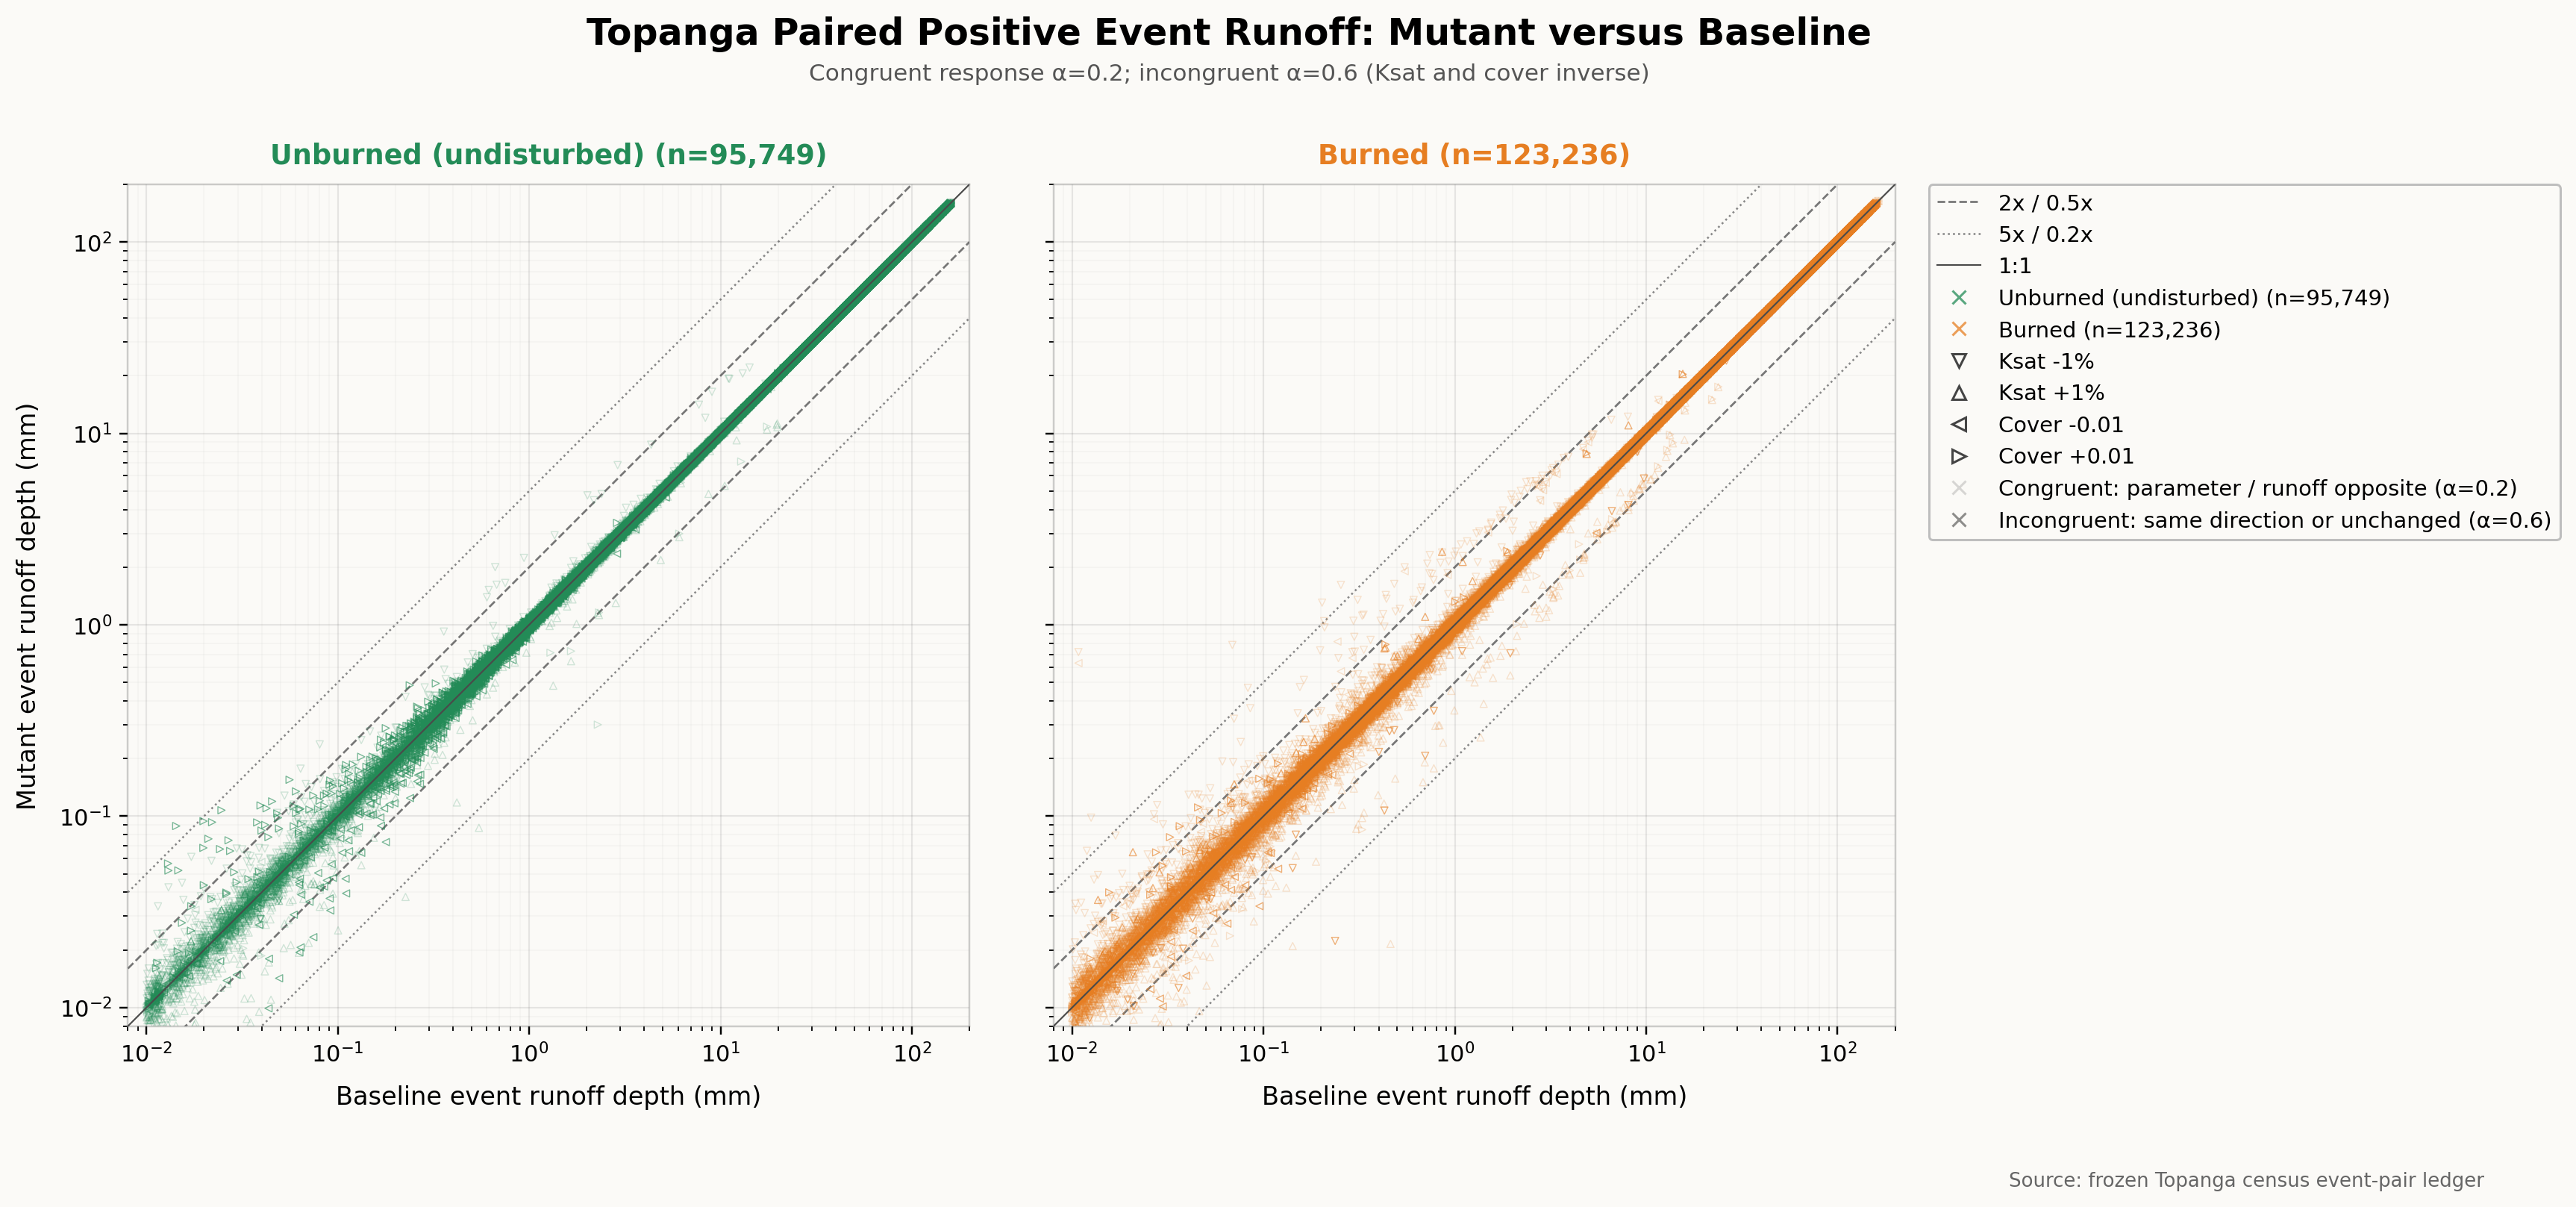
\includegraphics[width=\textwidth]{topanga-mutant-vs-baseline-runoff.png}
  \caption{Mutant versus baseline event runoff depth for 218,985
  paired-positive Topanga event rows. The population requires baseline runoff
  of at least 0.01 mm and positive mutant runoff. Unburned and burned strata
  occupy the left and right axes, respectively; triangle orientation identifies mutation family
  and direction. Faint markers are directionally congruent and dark markers
  are incongruent.}
  \label{fig:runoff-scatter}
\end{figure}

Only 451 runoff rows (0.21\%) lie outside the 0.5--2 ratio band, and only 36
(0.016\%) lie outside the 0.2--5 band. \Ksat{} accounts for 366 of the 451
twofold-tail rows (81.2\%) and 26 of the 36 fivefold-tail rows (72.2\%). These
tails exist, but they are both absolutely and proportionally smaller than the
corresponding peak-flow tails.

The separated panels confirm stable runoff in both strata. The twofold-tail
rate is 0.127\% for unburned rows and 0.267\% for burned rows; fivefold
departures remain rare at 0.014\% and 0.019\%, respectively.

Runoff direction is also strongly coherent for \Ksat{}. Overall, 146,131 of
218,985 runoff rows (66.7\%) are congruent. The \Ksat{} share is 111,359 of
113,242 rows (98.3\%), compared with 34,772 of 105,743 cover rows (32.9\%).
Exactly unchanged runoff is assigned to the incongruent display class; only
110 rows are exact ties.

This volume--peak contrast is central to the diagnosis. Under the same small
\Ksat{} probes, total event runoff is overwhelmingly stable and moves in the
ordinary hydrologic direction, while peak-flow magnitude contains the larger,
more structured extreme population. The evidence therefore points toward the
construction of subdaily runoff timing and peak rather than a comparable
instability in total event runoff depth.

\subsection{Event sediment delivery is mostly controlled but noisy}

Figure~\ref{fig:erosion-scatter} compares mutant and baseline WEPP event
sediment delivery (\texttt{Sed.Del}). This quantity is sediment delivered at
the hillslope outlet per unit width, not gross detachment across the hillslope.
The figure pairs records by scenario, hillslope, mutation, calendar year, and
day of year using the frozen Phase 2A baseline and census mutant event files.

\begin{figure}[H]
  \centering
  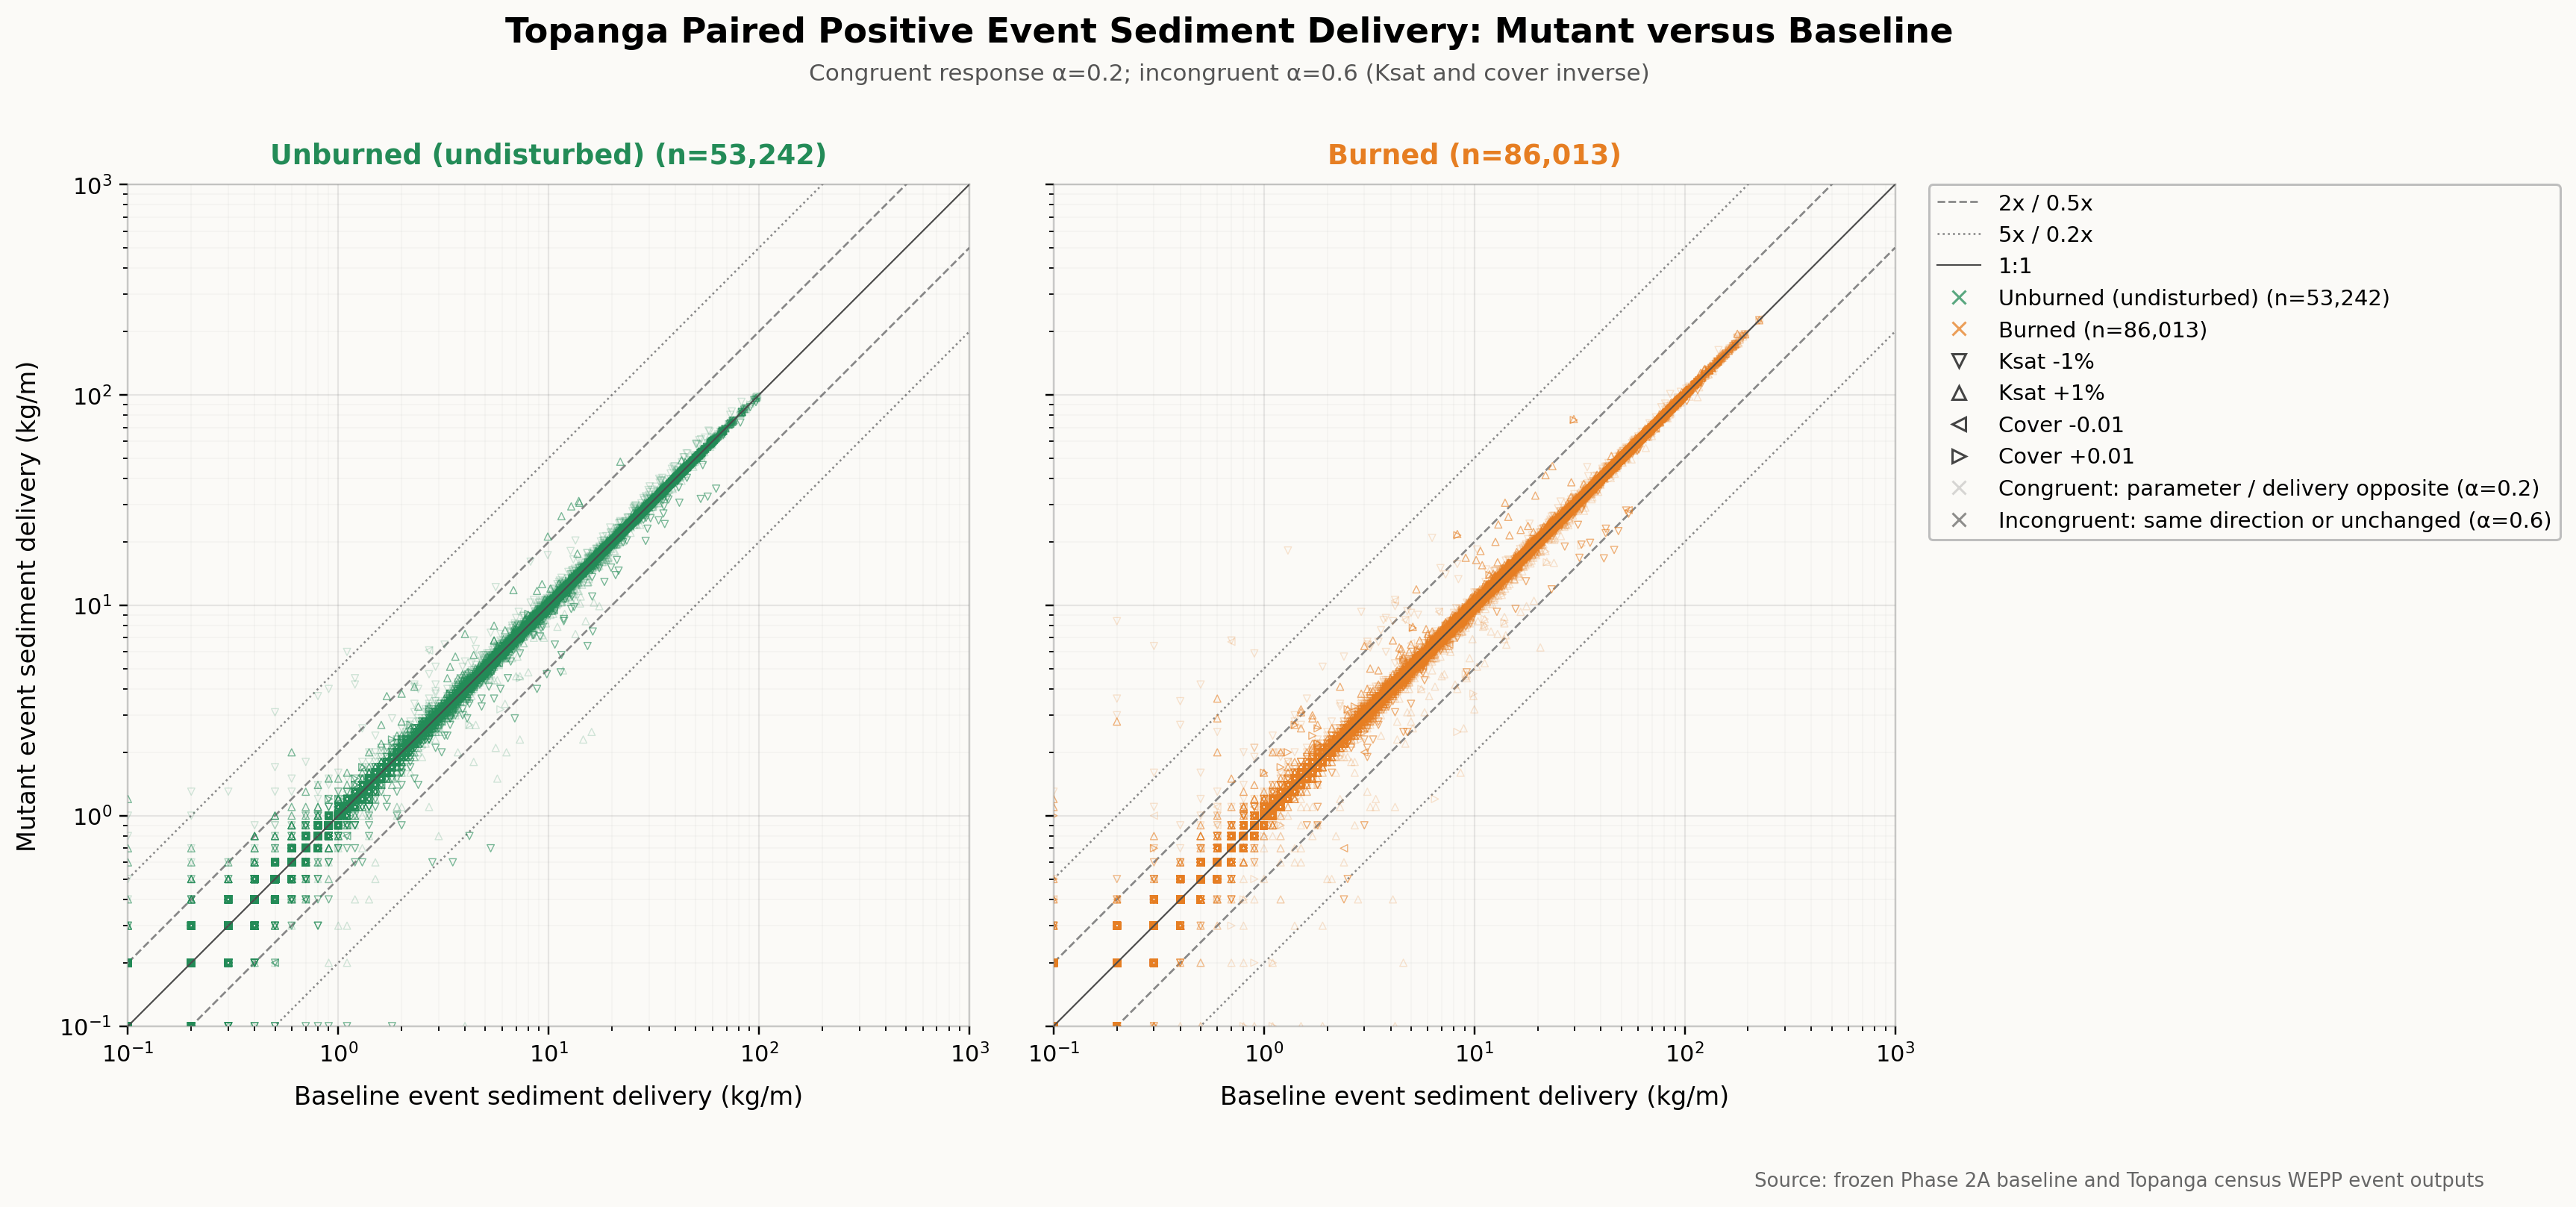
\includegraphics[width=\textwidth]{topanga-mutant-vs-baseline-erosion.png}
  \caption{Mutant versus baseline event sediment delivery for 139,255
  paired-positive Topanga event rows. Both axes use kg/m. Unburned and burned
  strata occupy the left and right axes, respectively; triangle orientation identifies
  mutation family and direction. Faint markers are directionally congruent
  and dark markers are incongruent. The stepped pattern at small magnitudes
  reflects the 0.1 kg/m precision of the retained WEPP event output.}
  \label{fig:erosion-scatter}
\end{figure}

Only 271 sediment-delivery rows (0.195\%) lie outside the 0.5--2 ratio band,
and only 55 (0.039\%) lie outside the 0.2--5 band. \Ksat{} accounts for 245 of
the 271 twofold-tail rows (90.4\%) and 49 of the 55 fivefold-tail rows (89.1\%).
The erosion response is therefore mostly controlled, and its material tail is
small and again concentrated in \Ksat{} mutations.

Twofold-tail prevalence is nearly identical after separating the strata:
0.203\% for unburned rows and 0.190\% for burned rows. Neither stratum's
material sediment-delivery tail was hidden by the other.

The central band should not be mistaken for precision. WEPP writes
\texttt{Sed.Del} to these retained files at 0.1 kg/m precision, producing
76,398 exact printed ties (54.9\% of paired-positive rows) and conspicuous
steps at small delivery. Relative differences near zero are consequently
noisy and less material in absolute terms. At moderate and large delivery,
the population remains concentrated near 1:1, but visible dispersion persists
within the 0.5--2 band. Event sediment-delivery values should therefore be
interpreted with an empirical factor-of-two sensitivity envelope in mind.
This envelope is descriptive of the Topanga small-mutation experiment; it is
not a formal statistical confidence interval or a universal WEPP uncertainty
bound.

Before the positive-delivery filter, event-date pairing produced 225,654 rows:
139,255 were positive in both runs, 505 were positive only in the baseline,
516 were positive only in the mutant, and 85,378 were positive in neither.
The one-sided and zero-delivery rows remain in the accounting but cannot be
displayed on logarithmic axes.

\subsection{Peak-flow magnitude distribution}

Figure~\ref{fig:scatter} shows the 199,086 paired-positive event rows. The dense
diagonal is the ordinary response population. Most events remain close to
baseline despite the high inclusive trial-screen prevalence. A sparse set of
points forms large upper and lower departures.

\begin{figure}[H]
  \centering
  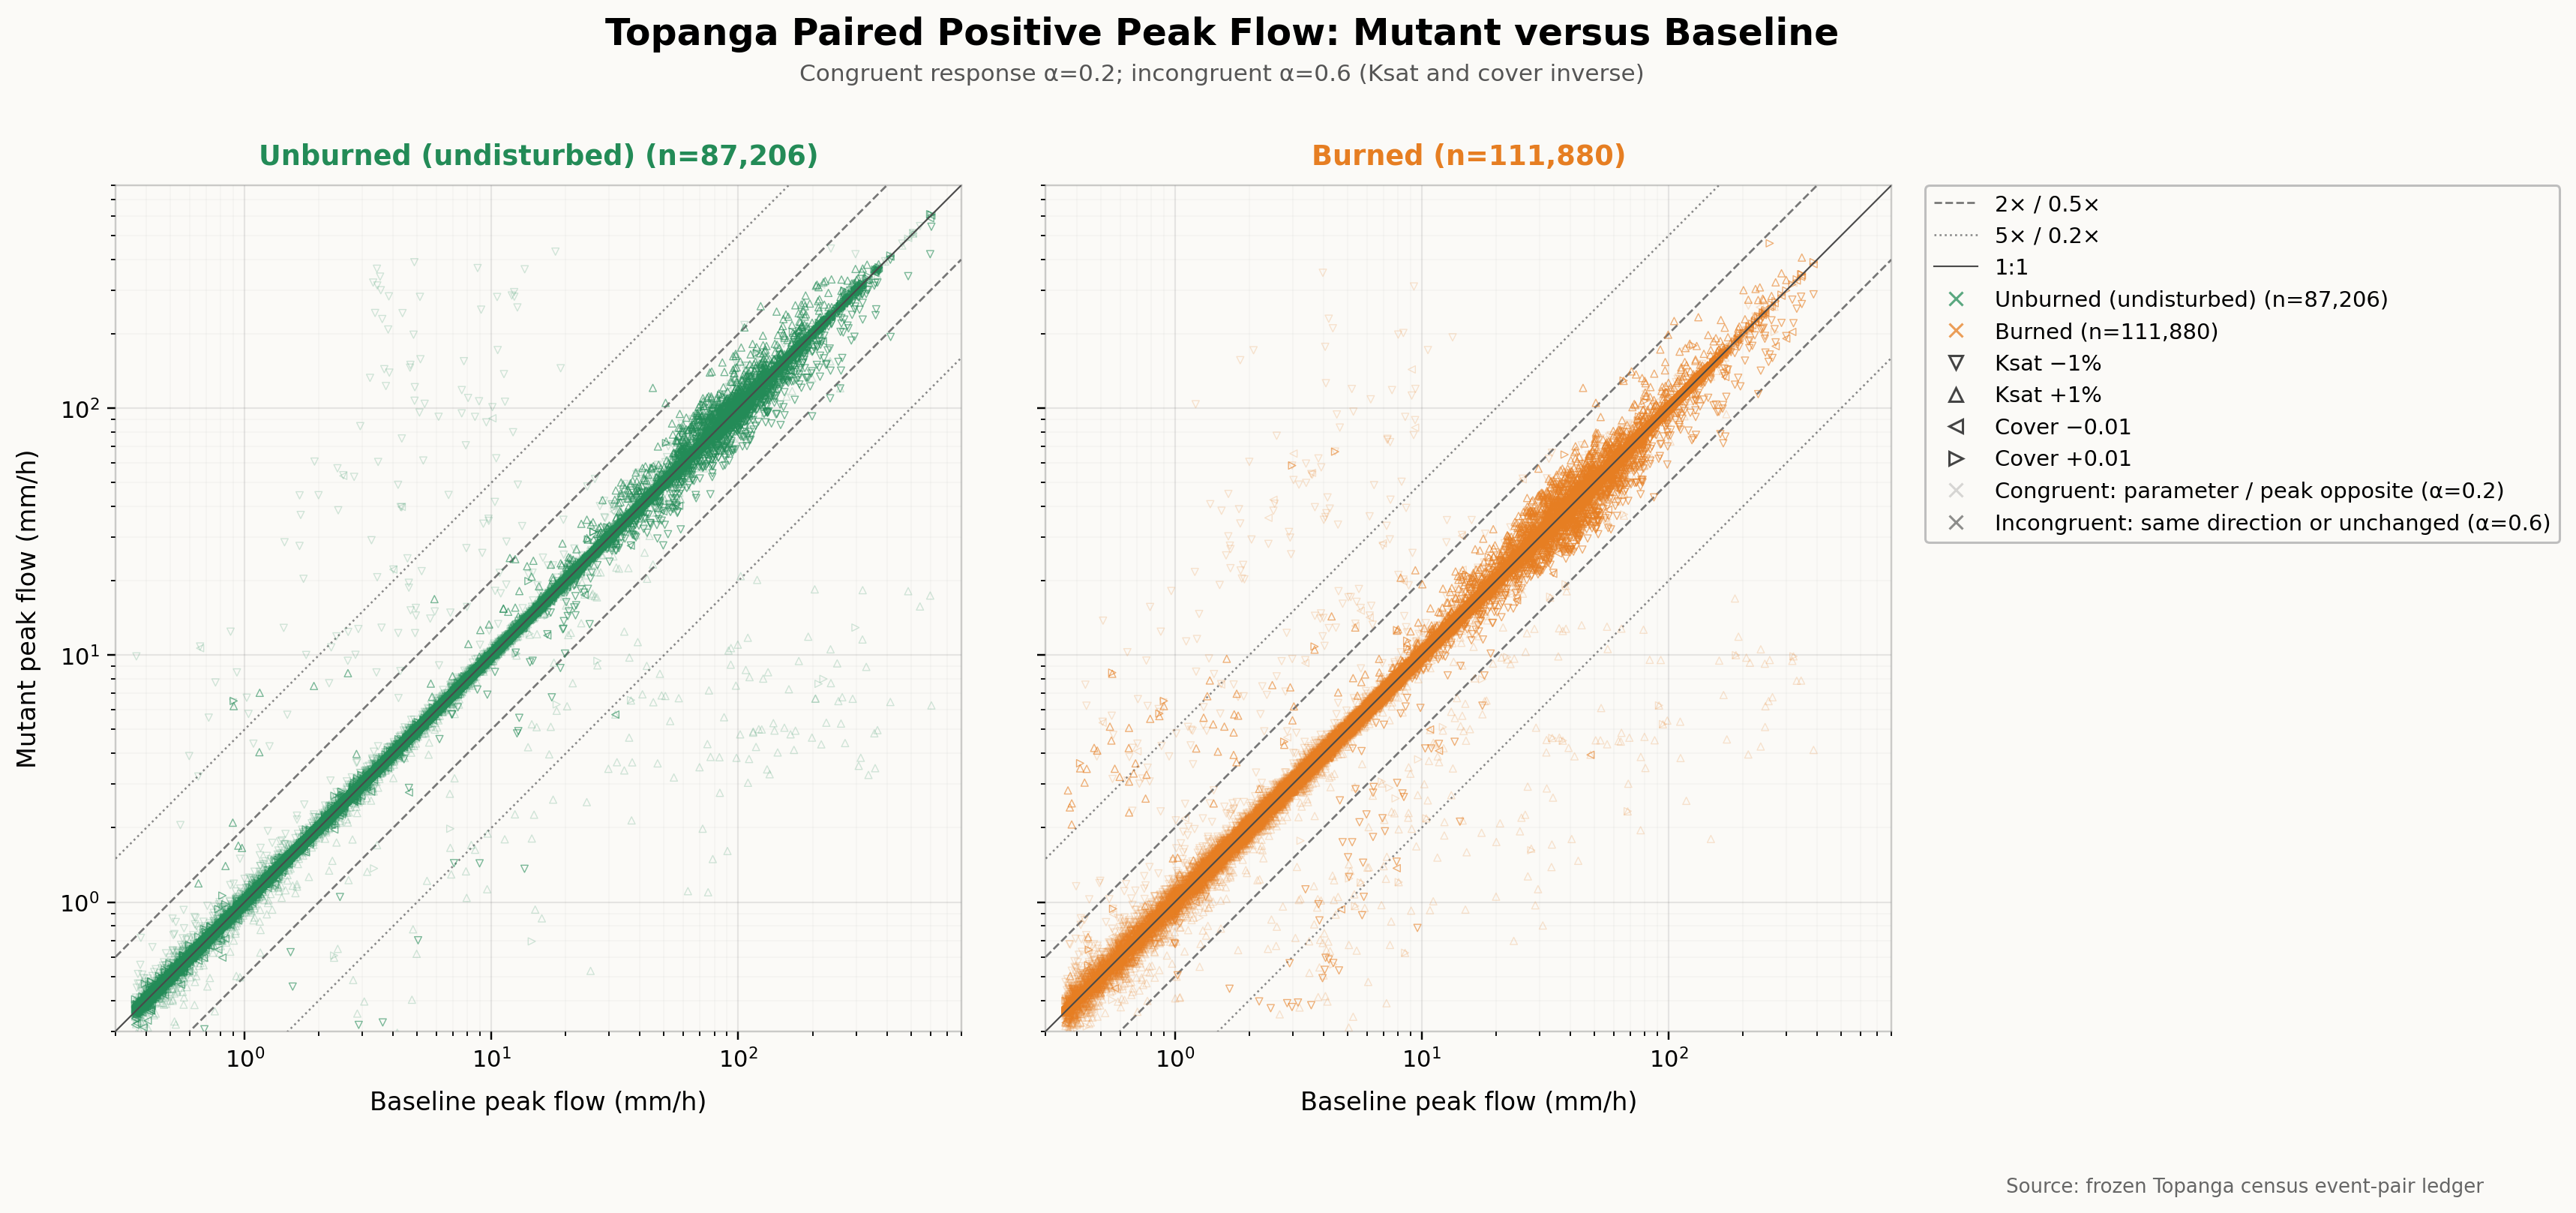
\includegraphics[width=\textwidth]{topanga-mutant-vs-baseline-peakflow.png}
  \caption{Mutant versus baseline hillslope peak flow for paired-positive
  Topanga event rows. Unburned and burned strata occupy the left and right axes.
  Green unburned and orange burned markers identify pairs with positive surface
  return in the baseline or mutant run; gray markers have no surface return in
  either run. Triangle orientation identifies mutation family and direction.
  Opacity identifies agreement with the ordinary inverse hydrologic response. The
  thin 1:1 line is drawn above the markers; dashed and dotted lines mark
  twofold and fivefold departures.}
  \label{fig:scatter}
\end{figure}

Surface return occurs in 81,904 of 87,206 unburned plotted rows and 74,026 of
111,880 burned rows. It is present in 567 of the 989 twofold-tail rows and 420
of the 604 fivefold-tail rows. Surface return therefore accompanies much of
the anomalous population, but it does not explain the entire tail: 422
twofold-tail rows and 184 fivefold-tail rows have no positive surface return in
either paired run. Most of that no-return tail is in the burned stratum. The
partition supports the documented surface-return timing mechanism for a large
part of the population while showing that additional peak-response mechanisms
must also be present.

Only 989 rows (0.50\% of the plotted population, approximately one in 201) lie
outside the 0.5--2 band, and 604 (0.30\%, approximately one in 330) lie outside
the 0.2--5 band. These tails are small but strongly structured:

\begin{table}[H]
  \centering
  \caption{Composition of the peak-ratio tails.}
  \label{tab:tails}
  \begin{tabular}{lrrrr}
    \toprule
    Ratio region & Rows & \Ksat{} rows & \Ksat{} share & Congruent share \\
    \midrule
    Outside 0.5--2 & 989 & 907 & 91.7\% & 79.0\% \\
    Outside 0.2--5 & 604 & 555 & 91.9\% & 83.8\% \\
    \bottomrule
  \end{tabular}
\end{table}

The dominant extreme response is therefore not a generic reaction to any small
input change. It is overwhelmingly associated with first-horizon \Ksat{}.
Most of these extreme \Ksat{} responses have the expected sign. The surprising
feature is their magnitude under a one-percent perturbation.

The separated panels show that the extreme branches occur in both strata. The
twofold-tail rate is 0.393\% for unburned rows and 0.577\% for burned rows;
the fivefold-tail rates are 0.280\% and 0.322\%, respectively. Burned conditions
have the higher tail prevalence, but the unburned extreme population is not an
overplotting artifact.

The split-stratum figure also locates the \Ksat{} response clusters at
different absolute peak magnitudes. Among directionally incongruent \Ksat{}
rows inside the 0.5--2 band, the median baseline peak is 74 mm/h in the
unburned stratum (interquartile range 50--103 mm/h) and 39 mm/h in the burned
stratum (26--51 mm/h). A separate magnitude criterion gives the same ordering:
among rows departing from baseline by more than 25\%, the median baseline peak
is 37 mm/h unburned and 10 mm/h burned. This displacement is not a climate
difference because corresponding burned and unburned hillslopes use identical
meteorological histories.

Pairing the same hillslope, mutation, year, day, OFE, and solver-call order
across strata further describes the shift. Of matched central-band \Ksat{}
rows, 1,164 are incongruent in both strata, 2,998 only in the unburned stratum,
and 7,204 only in the burned stratum. For the unburned-only group, median
baseline peaks are 72 mm/h unburned and 44 mm/h burned. For the burned-only
group, they are 38 mm/h burned and 9 mm/h unburned. The response regime is not
tied to one universal peak threshold. Soil, vegetation, cover, and
burn-severity parameterization shift the modeled hydrologic state at which the
unstable peak response is expressed. These are descriptive event-row
statistics; they do not identify the responsible state variable or solver
boundary.

\subsection{Directional agreement}

Across all plotted paired-positive rows, 64.1\% are directionally congruent.
The family-specific result is more informative: 87.4\% of \Ksat{} rows are
congruent, while only 39.2\% of cover rows are congruent.

\begin{table}[H]
  \centering
  \caption{Directional classification of paired-positive event rows.}
  \label{tab:direction}
  \begin{tabular}{lrrr}
    \toprule
    Population & Congruent & Incongruent & Congruent share \\
    \midrule
    Overall & 127,665 & 71,421 & 64.1\% \\
    \Ksat{} & 90,033 & 13,012 & 87.4\% \\
    Cover & 37,632 & 58,409 & 39.2\% \\
    Burned & 79,336 & 32,544 & 70.9\% \\
    Unburned & 48,329 & 38,877 & 55.4\% \\
    \bottomrule
  \end{tabular}
\end{table}

This correction is important for interpretation. The \Ksat{} tail does not
primarily show higher conductivity producing a higher surface-runoff peak.
Rather, small conductivity changes usually move peak flow in the expected
direction but sometimes produce an implausibly large change. Directional
congruence does not validate the magnitude.

\subsection{Incongruence increases with baseline peak within the central band}

The opacity pattern in Figure~\ref{fig:scatter} suggests more dark markers at
higher baseline peaks even within the 0.5--2 band. Direct tabulation confirms a
real conditional trend, especially for \Ksat{} (Table~\ref{tab:peakbins}). The
overall trend is not perfectly monotonic, but the high-flow bins are more often
incongruent than the low-flow bins.

\begin{table}[H]
  \centering
  \caption{Incongruent share within the 0.5--2 peak-ratio band, by baseline
  peak magnitude. The final bin contains only 145 rows and should be treated
  cautiously.}
  \label{tab:peakbins}
  \begin{tabular}{lrrr}
    \toprule
    Baseline peak (mm/h) & All families & \Ksat{} & Cover \\
    \midrule
    0.3--1 & 29.7\% & 1.2\% & 60.6\% \\
    1--3 & 34.7\% & 0.8\% & 72.1\% \\
    3--10 & 35.8\% & 1.7\% & 73.8\% \\
    10--30 & 31.6\% & 15.1\% & 48.3\% \\
    30--100 & 39.8\% & 25.4\% & 54.7\% \\
    100--300 & 43.6\% & 30.2\% & 57.4\% \\
    300--800 & 66.9\% & 52.9\% & 79.2\% \\
    \bottomrule
  \end{tabular}
\end{table}

Below 10 mm/h, \Ksat{} responses within the central
band are almost always directionally congruent. The incongruent share rises to
15.1\% at 10--30, 25.4\% at 30--100, and 30.2\% at
100--300 mm/h. This is not explained by cover,
which is frequently incongruent throughout the range and lacks the same clean
onset. It suggests that the local response regime changes with event magnitude
or with hydrologic states correlated with larger peaks.

The binning is descriptive. Event rows are clustered within trials and years,
and no independence-based significance test is claimed. Candidate mechanism
work should test whether this gradient aligns with surface-return depth,
positive-excess duration, forcing-mode changes, solver changes, or antecedent
profile state.

\section{Interpretation}

\subsection{What the Topanga census establishes}

The result has six levels:

\begin{enumerate}
  \item \textbf{Event runoff is stable.} The runoff scatter remains tightly
    concentrated around 1:1, and 98.3\% of \Ksat{} runoff responses have the
    expected direction.
  \item \textbf{Peak response separates from volume response.} The peak-flow
    tail is larger and more structured even though the corresponding runoff
    population remains tightly constrained.
  \item \textbf{Sediment delivery is mostly controlled but not exact.} Only
    0.195\% of paired-positive sediment-delivery rows depart by more than
    twofold, but low-magnitude quantization and central-band dispersion require
    a factor-of-two sensitivity envelope for event-level interpretation.
  \item \textbf{The extreme peak population is parameter-specific.} More than
    91\% of the twofold and fivefold tails are \Ksat{} mutations.
  \item \textbf{The main \Ksat{} concern is magnitude, not sign.} Most extreme
    \Ksat{} responses move in the hydrologically expected direction, but a
    one-percent change sometimes produces a many-fold peak change. Within the
    central band, wrong-sign \Ksat{} responses become more frequent as baseline
    peak increases.
  \item \textbf{Parameterization shifts the response regime.} Under identical
    climate histories, incongruent \Ksat{} responses cluster near substantially
    higher baseline peaks in the unburned stratum than in the burned stratum.
    The instability is conditioned on scenario-specific hydrologic state, not
    on a single absolute peak threshold.
\end{enumerate}

These observations are consistent with the known Hill 106 mechanism. \Ksat{}
changes infiltration, daily profile surplus, and the duration used to assign
that daily volume to a subdaily forcing. Near a duration or forcing-mode
boundary, a very small input change can be amplified. A solver branch can add
another discontinuity. The census does not prove that this exact sequence
explains every tail event, but it shows why \Ksat{} is the family in which the
extreme population should concentrate.

The between-stratum displacement adds a key finding: parameterization does not
merely change runoff and peak magnitude; it changes when the local peak-response
regime is entered. The known surface-return construction gives a plausible
implementation pathway because soil and cover affect infiltration, profile
surplus, and positive-excess duration. The census establishes the
state-dependent displacement, while candidate replay must determine which
duration, forcing-mode, or solver boundary explains each cluster.

\subsection{What changed after Chapter 4}

Chapter 4's statement that surface hydrology should perform best for large
events on one OFE described the model and evidence available in 1995. The
source history shows that the surface-return pathway now implicated in the
Topanga anomalies was not part of that evaluated calculation.

The source history changes how that claim should be judged. In 1993, WEPP
calculated excess water above the upper soil-water limit in a variable named
\texttt{surdra}. The source comments state that the water was not used because
runoff had already been routed and erosion had already been calculated. The
1995 documentation was therefore accurate when it said that return flow was
not explicitly represented. The surface-return pathway implicated at Topanga
was added later. A source comment dates S. Dun's initial \texttt{surdra}
runoff addback to May 22, 2003, with a modification on January 28, 2004.
Related comments date its integration with the peak-flow routine to June 6,
2003, with the no-duration handling extended on July 6, 2004. That code spreads
the daily returned-water volume across selected subdaily rainfall-excess
intervals before calculating the peak. On November 19, 2009, the call to the
daily water balance was moved inside the peak-flow routine; the accompanying
comment notes that this differed from WEPP's original sequence and might affect
other global variables \cite{stakeholder}.

\begin{table}[H]
  \centering
  \small
  \caption{Source-supported history of the surface-return pathway.}
  \label{tab:surdra-history}
  \begin{tabular}{lp{0.67\textwidth}}
    \toprule
    Date & Source evidence and meaning \\
    \midrule
    May 1993 & \surdra{} calculated but explicitly unused because runoff routing and erosion had already occurred \\
    July 1995 & Chapter 4 published with return flow outside the documented formulation \\
    May 22, 2003 & Initial \surdra{} runoff addback \\
    June 6, 2003 & Integration with the peak-flow routine \\
    January 28, 2004 & Surface-return addback modified \\
    July 6, 2004 & No-duration handling extended \\
    November 19, 2009 & Daily water balance moved inside the peak-flow routine \\
    2026 & Topanga population-scale mutation census \\
    \bottomrule
  \end{tabular}
\end{table}

This history is supported by source-code forensics. The dated comments show
what the developers calculated, what they deliberately left unused, and when
the later addback and sequencing changes appeared. That evidence is not
available from the model output or the 1995 documentation alone. It was
possible to identify the Topanga defect because unofficially preserved WEPP
source copies could be compared and instrumented. USDA has distributed WEPP
primarily as an executable and has not provided users with an official,
complete release of the production source. Most WEPP users therefore cannot
inspect this calculation, trace a surprising peak through the program, or see
that the documented performance claim predates the surface-return code.

Stone et al.'s favorable claim could therefore have been true for the 1995
model they evaluated. This study does not have a 1995 executable and does not
test that historical version. What the Topanga census refutes is the continued
use of the 1995 claim as assurance about the present implementation. On the
current single-OFE hillslopes, the incongruent share of central-band \Ksat{}
responses increases rather than decreases with baseline peak magnitude, and a
one-percent change can produce a many-fold peak change while runoff remains
nearly fixed. The large events most relevant to frequency analysis are not the
most dependable individual peak estimates in the current model.

The most likely history is straightforward. A later development change added
a useful water-balance pathway that the original developers had deliberately
left unresolved because of its timing within the daily calculation. That
change altered the water supplied to the peak-flow calculation, but the peak
method and its performance guidance were not reevaluated at population scale.
The Chapter 4 statement remained in the documentation even though the model
around it had changed. In that sense, the documentation became stale: it
continued to describe the scope and evidence of the 1995 peak calculation, not
the behavior of the later surface-return implementation. Limited access to the
source made that mismatch much harder for users to recognize.

The historical omission is understandable. The original developers evaluated
the approximation using the theory, selected cases, data, and computing
resources available in the early 1990s. A census of hundreds of thousands of
paired event responses would have been impractical. The Topanga census applies
modern computing to a validation question that appears not to have been asked
after the surface-return pathway was added. Its contribution is not to show
that Stone et al. were wrong in 1995. It is to show that a later model change
invalidated the assumption that their original performance claim still applied.

\subsection{Production-scale implication}

The small tail fraction does not make an individual modeled peak dependable.
The Topanga census found 604 paired-positive event rows outside the 0.2--5
ratio band, an empirical rate of approximately one in 330. This is an
event-row rate within an enriched-discovery site, not an independent-event
probability and not a universal WEPP defect rate. Nevertheless, production
watersheds can contain thousands of hillslopes evaluated over thousands of
events. At that scale, even a sparse local tail provides many opportunities
for one hillslope or a small group of hillslopes to contribute an abnormal
peak. The risk is not confined to the conspicuous many-fold tail. Within the
nominally central 0.5--2 ratio band, directional incongruence increases with
baseline peak magnitude, especially for \Ksat{}. The \Ksat{} incongruent share
rises from 1.7\% at baseline peaks of 3--10 mm/h to 15.1\% at 10--30 mm/h,
25.4\% at 30--100 mm/h, 30.2\% at 100--300 mm/h, and 52.9\% at
300--800 mm/h. The final bin contains only 145 total event rows and is
therefore uncertain, but the broader increase begins well below it. Thus, the
events most capable of influencing an upper-tail frequency analysis are also
the events for which the expected local response becomes less dependable.

This magnitude-conditioned incongruence is distinct from the far-tail result.
Most responses outside the 0.5--2 and 0.2--5 bands are directionally
congruent; their problem is a disproportionate magnitude under a one-percent
probe. Within the central band, the additional concern is that larger events
increasingly move in the unexpected direction. Production return-period
estimates may therefore be exposed both to rare many-fold peak anomalies and
to a broader, peak-dependent instability among events that remain within a
factor of two of baseline.

This distinction changes the practical interpretation. The population-level
response is mostly sensible, but a particular hillslope-event peak cannot be
presumed reliable merely because most rows lie near 1:1. Extreme-value
statistics are especially vulnerable because a few unusually large values can
alter exceedance ranks, fitted tails, and estimated return periods. A plausible
production mechanism is therefore that rare abnormal hillslope peaks propagate
into aggregated peak-flow statistics and distort reported return periods.
Topanga demonstrates the anomalous hillslope-scale source term; because the
census intentionally omitted per-mutation watershed routing, the downstream
propagation and return-period effect remain a specific hypothesis requiring
routed replay and production-run audit.

\subsection{Why larger mutations are not presently needed}

The purpose of the mutation is to interrogate continuity near the operational
baseline, not to span a plausible calibration range. The $\pm1\%$ \Ksat{} and
$\pm0.01$ cover probes already provide:

\begin{itemize}
  \item a large paired event population;
  \item a dense ordinary-response reference population;
  \item clearly separated tails;
  \item strong family attribution; and
  \item known-positive events suitable for bracketing and replay.
\end{itemize}

Increasing the mutation magnitude would make it harder to distinguish a local
implementation discontinuity from an ordinary nonlinear physical response. A
larger bracket is useful only after a small probe flags a candidate and the
candidate is examined adaptively. For cross-site screening, the same small
matrix should remain the default.

\subsection{Do not assume the undisturbed result is the known result}

When hydrologists compare burned and undisturbed simulations, we usually treat
the undisturbed run as the control. If the burned run gives an unexpected
answer, we first question the burn-severity map or the postfire soil and cover
values. We rarely begin by asking whether the undisturbed result is the one
that is wrong. Topanga shows why that habit can mislead us.

The burned model is, in some ways, the more tightly constrained model. A
remotely sensed soil-burn-severity map tells us where the fire effects occurred
and how severe they were. The WEPP postfire soil and cover values are based on
rainfall-simulation experiments. These observations do not make the burned
model perfect, but they give it a spatial and experimental basis.

The undisturbed model does not have an equivalent map of the watershed's
hydrologic condition. Before the fire, Topanga contained a complicated mixture
of chaparral, shrubs, grass, litter, roots, and vegetation growing in and near
channels. These plants intercept rain and remove water from different depths
and at different times of year. The undisturbed Omni scenario reduces much of
that variation to one general representation. In other words, ``undisturbed''
is the name of a modeled condition. It does not mean that the condition is
known more accurately.

The 2020 water balance gives a reason to question that baseline
\cite{handoff}. With the restrictive layer removed and PMET $K_{cb}=1.20$, the
complete undisturbed watershed produced 149.68 mm of routed outlet flow. The
available gauge record corresponds to about 6.2 mm. Those numbers are not
directly comparable: the gauge and model boundaries differ, and the gauge
includes all sources and losses. The observation is only a magnitude check.
Even so, the difference is too large to support the assumption that the
undisturbed run is a well-established control. Removing the restrictive layer
did not solve the discrepancy. It moved water from lateral flow into deep
percolation and groundwater return. Changing $K_{cb}$ also had little effect on
the event peaks.

The mutation study points in the same direction. As the computed undisturbed
peak flow becomes larger, the response to a very small \Ksat{} change becomes
more scattered and more often moves in the wrong direction. This pattern
occurs at higher peak flows in the undisturbed run than in the burned run.
These results do not prove that the real undisturbed watershed is noisy. They
show that the model's large undisturbed peaks are not a stable reference.

This changes how a burned-versus-undisturbed inversion should be investigated.
If the burned peak is lower than the undisturbed peak, the first question
should not automatically be, ``What is wrong with the burned model?'' The
undisturbed peak may be abnormally high. Both results need to be checked, and
at Topanga the undisturbed result deserves at least as much scrutiny as the
burned result. The central lesson is simple: the prefire scenario is a
comparison case, not ground truth.

\section{Limitations and Claim Boundary}

\paragraph{What is established.}
The documentation, source comparison, diagnostic execution, and census jointly
establish that:

\begin{itemize}
  \item present WEPP assigns a daily \surdra{} depth new subdaily timing rather
    than routing the hourly return series;
  \item that operation caused the 1980 \Ksat{} peak reversal, while the solver
    switch enlarged but did not create the reversal;
  \item controlled canopy and cover changes expose additional repeatable peak
    discontinuities;
  \item the Topanga population contains a structured, predominantly
    \Ksat{}-associated extreme tail; and
  \item runoff volume is substantially more stable than calculated peak rate.
\end{itemize}

\paragraph{What remains unresolved.}
The evidence does not establish that every extreme row has the same cause.
Positive surface return occurs in 567 of 989 twofold-tail rows and 420 of 604
fivefold-tail rows, leaving a material no-return tail, especially in the
burned stratum. The immediate branch behind the 1986 cover boundary is not yet
known; neither side of an extreme pair has been established as the physically
correct peak; and the Windows source comparison is static rather than a fully
instrumented execution of every Topanga fixture. Watershed routing and effects
at the outlet also remain outside this census.

\paragraph{Study-scope limitations.}

\begin{itemize}
  \item \textbf{One enriched-discovery site.} Topanga was selected because it
    contained known anomalies. These rates are not cross-site prevalence
    estimates.
  \item \textbf{Event-row clustering.} A trial contributes many events.
    Event-row percentages are not percentages of independent hillslopes,
    storms, or watersheds.
  \item \textbf{Inclusive screening.} A candidate can be triggered by event
    appearance, solver change, directional reversal, magnitude change, or
    surface-return-rate change. Candidate prevalence is not confirmed-defect
    prevalence.
  \item \textbf{Local hillslope scope.} Per-mutation watershed routing was
    intentionally removed after the pilot exposed unresolved off-path changes
    and incompatible channel-volume authorities. No attenuation, synchronization,
    or outlet-impact claim is made.
  \item \textbf{Positive-event magnitude figures.} The peak scatter excludes
    rows below the baseline peak floor or without a positive mutant peak. The
    runoff scatter similarly applies the 0.01 mm baseline runoff floor and
    requires positive mutant runoff. The sediment-delivery scatter requires
    positive delivery on both sides; its zero and one-sided rows are reported
    separately. Event-presence changes remain in the complete ledger and
    candidate screen.
  \item \textbf{Sediment-output precision.} The retained event files report
    sediment delivery to 0.1 kg/m. Exact ties and low-magnitude relative noise
    therefore include output quantization, not solely model response.
  \item \textbf{Mechanisms not exhaustively adjudicated.} Hill 106 establishes
    implementation mechanisms that can produce discontinuity. The full tail
    population still requires trial-level grouping, adaptive bracketing, and
    frozen-event replay.
\end{itemize}

\section{Next Steps}

\subsection{Additional sites}

The next sites should retain the exact small-mutation design, execution
contract, floors, and event-pairing keys. Site selection should proceed under
the two preregistered portfolios already defined by the audit:

\begin{itemize}
  \item \textbf{Enriched discovery}: known-positive rain-dominated sites such
    as Palisades and Stevens Canyon, used to test recurrence of known mechanisms.
  \item \textbf{Blind audit}: sites frozen by hydrologic and provenance criteria
    before their peak responses are examined.
\end{itemize}

The portfolio should add rain-dominated forest, transient-snow, and
snow-dominated forest conditions. Results must be reported separately for
enriched and blind portfolios. A shared small-probe design makes the site
comparison interpretable; increasing mutation size at later sites would change
the estimand.

\section{Conclusion}

The Topanga census demonstrates why small-mutation screening is valuable. A
large perturbation was not required to reveal the issue. Under $\pm1\%$ \Ksat{}
and $\pm0.01$ paired-cover probes, most paired events remain near baseline,
providing a clear ordinary-response reference. Event runoff is especially
stable: 98.3\% of \Ksat{} runoff responses have the expected direction, and
only 0.21\% of plotted runoff rows depart by more than twofold. Event sediment
delivery is also mostly controlled: 99.805\% of paired-positive rows remain
within a factor of two. Its low-magnitude values are quantized and noisy, and
the visible central-band dispersion supports interpreting individual erosion
outputs with an empirical factor-of-two sensitivity envelope rather than as
precise event predictions.

Against the stable runoff-volume response, a small but conspicuous peak-flow
extreme population appears. It is overwhelmingly associated with \Ksat{},
usually moves in the expected hydrologic direction, and is too large to
summarize as ordinary local sensitivity to a one-percent change. The 604 rows
outside the 0.2--5 band represent an empirical Topanga rate of approximately
one in 330 paired-positive event rows. Thus, the peak calculation is sensible
in aggregate but cannot be trusted without qualification for an arbitrary
hillslope event. Topanga definitively demonstrates that the diagnostic
peak-flow calculation can generate anomalous peaks of meaningful magnitude at
hillslope scale.

The burned--unburned separation supplies an additional key result. Because the
two strata share the same climate sequence, the shift from an unburned \Ksat{}
incongruence cluster near 74 mm/h to a burned cluster near 39 mm/h reflects the
effect of soil, vegetation, cover, and burn-severity parameterization on the
modeled hydrologic state. Parameterization changes not only runoff magnitude
but the peak scale at which the unstable response regime is encountered. This
state shift provides a credible link to previously observed burned--unburned
peak inversions: scenario-specific events can enter the amplified peak regime
at different points even under the same storm forcing. The association is
demonstrated here; attribution to a particular duration or solver transition
still requires frozen-event replay.

In production, a single hillslope or a small set of hillslopes may contribute
abnormal events that distort aggregated extremes and return-period estimates.
That pathway is operationally credible given the empirical tail rate and the
large hillslope-by-event population of a production run. It remains an
inference, however, until routed replays show how the hillslope anomalies
propagate to watershed outputs and affect fitted return periods.

The appropriate next step is replication, not expansion of mutation magnitude.
Apply the same small design at additional preregistered sites, preserve the
Topanga claim boundary, and mechanism-trace selected candidates. Until that
work is complete, the report supports a local Topanga finding: WEPP hillslope
peak flow contains a structured \Ksat-sensitive response whose magnitude and
state dependence warrant implementation-level investigation.

\section*{Evidence and Reproducibility}

The principal local sources for this report are:

\begin{itemize}
  \item the Topanga investigation handoff, including the Windows reconstruction
    and Hill 106 mechanism narrative;
  \item the stakeholder report on WEPP peak-flow documentation and Topanga
    implementation evidence;
  \item the multi-site audit protocol and its local-census amendment;
  \item the frozen Topanga execution disposition and prevalence summary; and
  \item the figures, sidecars, plotting scripts, and repeatable stratum-cluster
    analysis under the Topanga execution work package.
\end{itemize}

Two diagnostic stages should not be confused. The original Hill 106 mechanism
trace and forced-solver tests used WEPP-Forest source commit
\texttt{2f65506d239b449b...fa55158} and executable \texttt{wepp\_260803}.
The later census observer used commit \texttt{ea25ad79} and recorded every
peak-solver call without changing ordinary WEPP outputs. The public Windows
comparison used Daily Erosion Project commit
\texttt{e2609d9e67757f...ef657c}, whose \texttt{src/wepp20240930} directory is
recorded as a verbatim September 2024 WEPP import. Public implementation links,
complete hashes, and file comparisons are retained in the stakeholder evidence
report \cite{stakeholder}.

The source-code evidence is essential to the defect identification. Ordinary
WEPP output does not expose the daily return depth, selected duration, imposed
rate, ponding-time sentinel, or solver handoff. USDA has distributed WEPP
primarily as an executable and has not provided an official complete release
of the production source. The analysis was possible because preserved source
copies could be compared, instrumented, and checked against unchanged model
outputs.

The figure source is
\path{docs/work-packages/20260809_peakflow_topanga_census_execution/artifacts/}.
The immutable event ledger is inventoried by the execution package's external
evidence manifest. The report deliberately cites compact repository evidence
rather than embedding the large Parquet ledger.

\begin{thebibliography}{9}

\bibitem{stone1995}
Stone, J. J., Lane, L. J., and Shirley, E. D. (1995).
``Hillslope Surface Hydrology.'' In \emph{USDA--Water Erosion Prediction
Project: Hillslope Profile and Watershed Model Documentation}, Chapter 4,
NSERL Report No. 10.
\url{https://www.ars.usda.gov/ARSUserFiles/50201000/WEPP/chap4.pdf}.

\bibitem{savabi1995}
Savabi, M. R., Skaggs, R. W., and Onstad, C. A. (1995).
``Subsurface Hydrology.'' In \emph{USDA--Water Erosion Prediction Project:
Hillslope Profile and Watershed Model Documentation}, Chapter 6,
NSERL Report No. 10.
\url{https://www.ars.usda.gov/ARSUserFiles/50201000/WEPP/chap6.pdf}.

\bibitem{stakeholder}
Lew, R. and agentic collaborators (2026).
``WEPP Peak-Flow Estimation: Long-Standing Discontinuities and Their
Implementation Basis.''
\path{docs/investigations/2026-08-07-topanga-2025-fire-peak-flow-analysis/artifacts/wepp-peak-flow-solver-documentation-and-topanga-evidence.md}.

\bibitem{handoff}
Lew, R. and agentic collaborators (2026).
``Topanga Investigation Handoff.''
\path{docs/investigations/2026-08-07-topanga-2025-fire-peak-flow-analysis/artifacts/bill-windows-replication-handoff.md}.

\bibitem{audit}
WEPP Peak-Flow Discontinuity Multi-Site Audit (2026).
\path{docs/investigations/2026-08-08-wepp-peak-flow-discontinuity-multi-site-audit/README.md}.

\bibitem{disposition}
Frozen Topanga Local Census Execution Disposition (2026).
\path{docs/work-packages/20260809_peakflow_topanga_census_execution/artifacts/execution-disposition.md}.

\end{thebibliography}

\end{document}
